% ============================================================
%  CAPÍTULO 4 — RESULTADOS Y DISCUSIÓN  (reescritura thesisV2, sin Enfoque A)
% ============================================================
\chapter{Resultados y Discusión}
\label{cap:resultados}

Este capítulo presenta los resultados sobre la base de datos oficial: las
sesiones S2--S7 (6 sesiones, 14\,901 ventanas de $128\times128$~px), con
\textbf{487 ventanas positivas} (centro dentro del bounding box de la \ac{MAP})
y \textbf{14\,414 negativas}, un desbalance real de \textbf{30:1}. Todas las
métricas se obtienen con validación \ac{LOSO} (\emph{dejar una sesión fuera}).
Para corregir ese desbalance 30:1, el conjunto de entrenamiento se balancea con
\textbf{submuestreo aleatorio~1:1} dentro de cada pliegue, conservando la sesión
de prueba con su distribución real.

El hilo del capítulo es: (1)~caracterizar la firma espectral de cada clase;
(2)~validar que el cálculo de índices a nivel de imagen equivale al de ventana;
(3)~identificar qué características son discriminativas; (4)~elegir el
clasificador; (5)~reducir el número de características; (6)~reportar el modelo
final; y (7)~analizar su comportamiento por sesión, profundidad y falsos
positivos.

% -------------------------------------------------------------
\section{Firmas espectrales por clase}
\label{sec:firmas}

\textbf{Objetivo.} Analizar visualmente la capacidad discriminativa de las bandas
espectrales que captura la cámara y de los índices derivados de ellas, para verificar
---\emph{antes de entrenar ningún clasificador}--- si la \ac{MAP} se distingue de los
objetos de interferencia (botella, lata, piedra) y del control.

\textbf{Metodología.} Cada ventana se asigna a una clase según dónde cae su
centro (bounding box de Roboflow para \ac{MAP}, botella, lata y piedra; zona de
control para Control). Para cada clase se observa la \emph{distribución} de la
reflectancia por banda y de los índices, mediante diagramas de violín que
permiten comparar las clases entre sí y evaluar su separabilidad visual.

\begin{figure}[H]
  \centering
  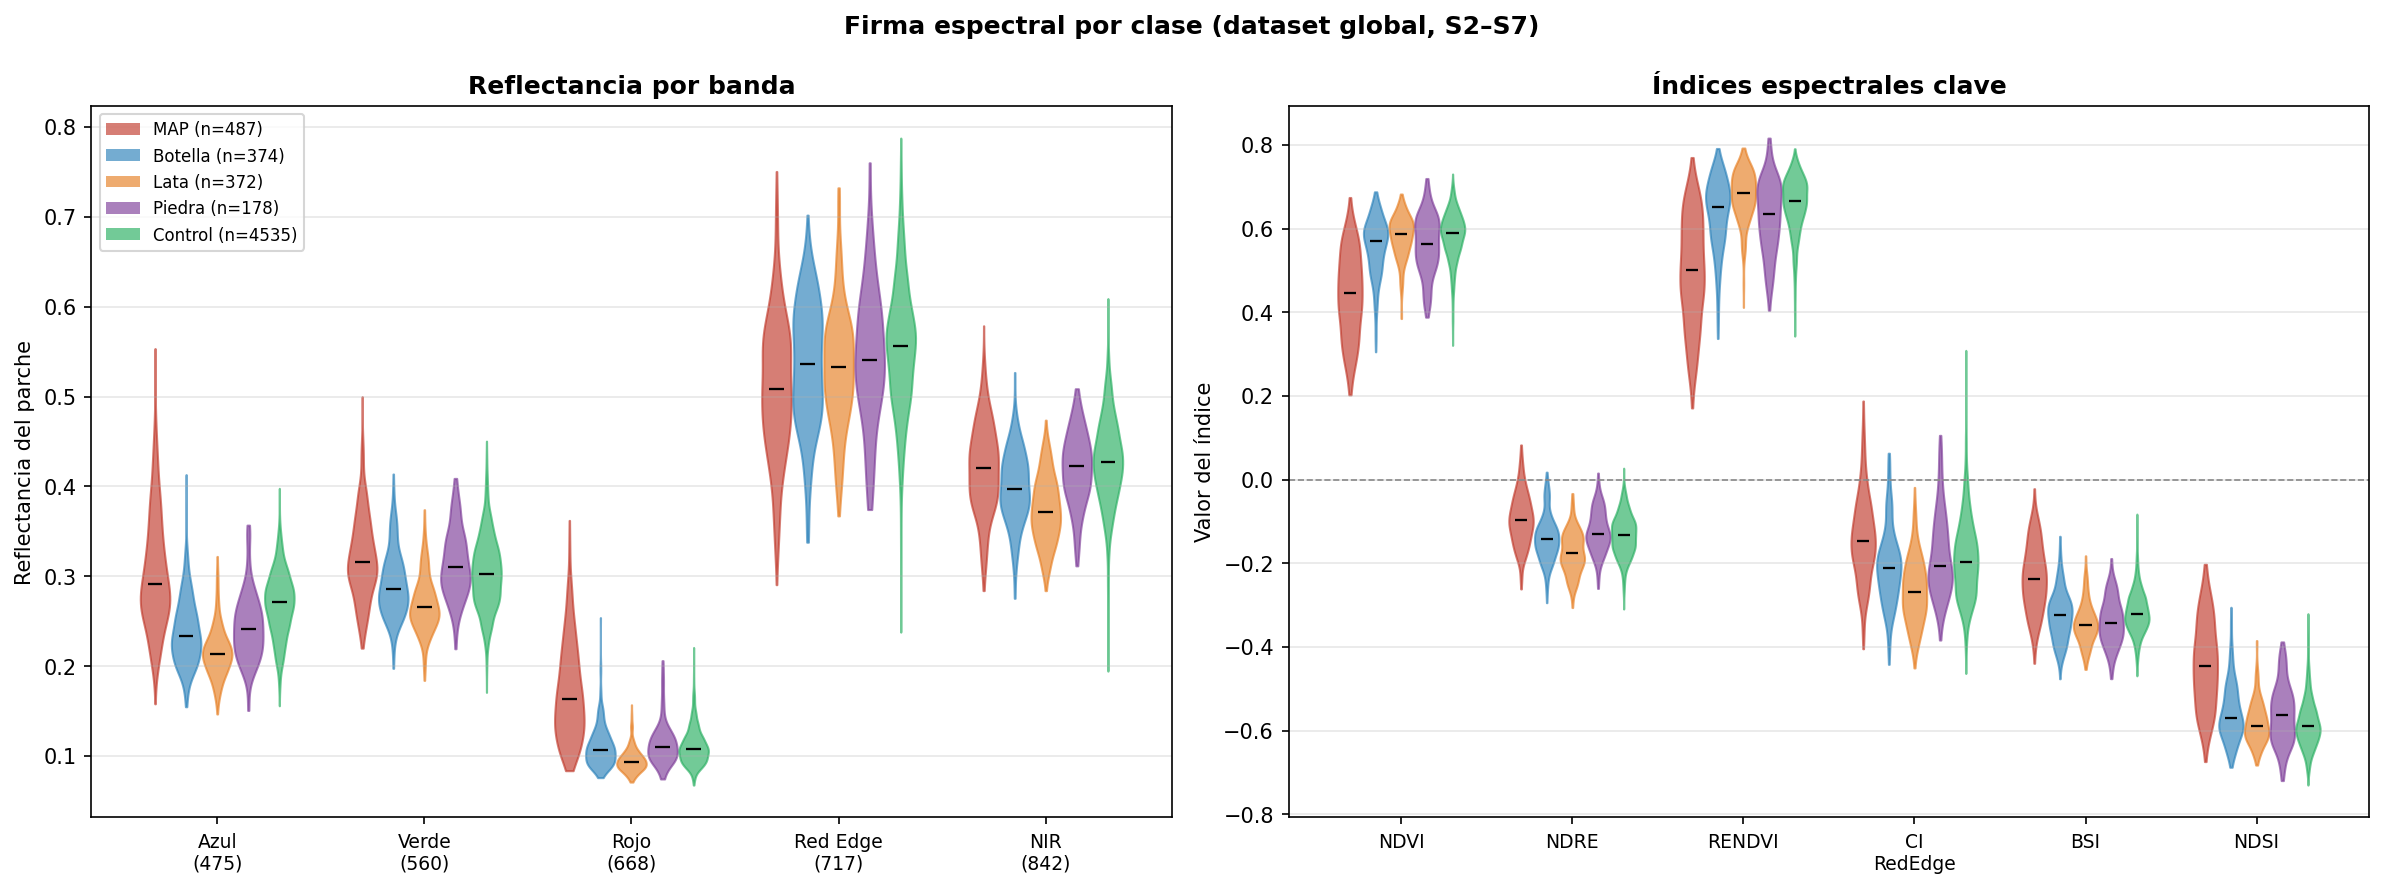
\includegraphics[width=\textwidth]{figuras/p1_violin_firma.png}
  \caption{Distribución de la firma espectral por clase (S2--S7).
    \textit{Izquierda:} reflectancia por banda. \textit{Derecha:} índices
    espectrales clave. Conteos: \ac{MAP}~=~487, Botella~=~374, Lata~=~372,
    Piedra~=~178, Control~=~4\,535.}
  \label{fig:firmas}
  \label{fig:firmas_espectrales}

  {\footnotesize Fuente: elaboración propia.}
\end{figure}

\textbf{Resultados y análisis.} En la Figura~\ref{fig:firmas}, cada violín es la
\emph{distribución} de una clase: su ancho indica dónde se concentran las ventanas
(más ancho, valores más frecuentes) y la línea negra marca la mediana; lo relevante
es comparar la altura del violín de la \ac{MAP} (rojo) con la de las demás clases.
Bajo ese criterio, en el panel de reflectancia la \ac{MAP} es la clase de
\emph{mayor} reflectancia, de forma marcada en el \textbf{Rojo} (mediana
$0.157$ frente a $\sim$$0.10$ en las demás), coherente con el suelo desnudo del
área perturbada por el enterramiento; en Azul y Verde la diferencia respecto a
Control es pequeña, así que la discriminación visible se concentra en el Rojo.
En los índices, el \textbf{NDVI} es el que más separa a la \ac{MAP} (valores
bajos por la menor cobertura vegetal activa), seguido de \textbf{NDSI} y
\textbf{RENDVI}; el NDRE y CI\_RedEdge separan menos.

No existe un índice que separe a la \ac{MAP} de forma perfecta: los violines se \emph{solapan parcialmente}. De
hecho, entre el 18\,\% y el 24\,\% de las ventanas con \ac{MAP} caen dentro del
rango intercuartil de las otras clases en NDVI. Esto anticipa que la separación
a nivel de ventana individual no será perfecta (habrá falsos positivos y
negativos) y justifica usar un clasificador que combine muchas características en
lugar de un solo índice. Los índices que aquí destacan (NDVI, NDSI, RENDVI)
reaparecerán en el análisis de importancia (Sección~\ref{sec:importancia}),
confirmando esta primera lectura.

% -------------------------------------------------------------
\section{Cálculo de índices: imagen completa vs ventana}
\label{sec:indices_global}

\textbf{Objetivo.} Evaluar si calcular los índices una sola vez sobre la imagen
completa ---y extraer después las estadísticas por ventana--- produce el mismo
resultado que recalcularlos dentro de cada ventana, y observar la diferencia en
el costo de cómputo entre ambas formas.

\textbf{Metodología.} Se extrajeron las 378 características de las dos formas
---\emph{ventana} (recalcula los índices en cada parche) y \emph{global}
(índices una vez sobre la imagen, estadísticas por ventana)--- con idéntica
semilla, y se compararon numéricamente, en métricas \ac{LOSO} (\ac{RF}, 1:1) y
en tiempo de extracción.

\textbf{Resultados.} Las características resultan \textbf{idénticas bit a bit}
($\max|\text{global}-\text{ventana}| = 0$ sobre las 378 columnas), por lo que las
métricas \ac{LOSO} coinciden exactamente (Tabla~\ref{tab:indices_modo}). El modo
global es $\sim$9\,\% más rápido en extracción.

\begin{table}[H]
\centering
\caption{Equivalencia entre el cálculo de índices por ventana y a nivel de imagen
         (\ac{RF}, 378 características, \ac{LOSO}, 1:1).}
\label{tab:indices_modo}
\small
\begin{tabular}{lccccc}
\toprule
\textbf{Modo} & \textbf{AUC} & \textbf{Sens(0.5)} & \textbf{Spec(0.5)} &
\textbf{FP/mina} & \textbf{Tiempo extracción} \\
\midrule
Ventana (por parche) & 0.915 & 0.805 & 0.856 & 5.29 & 1856 s \\
\textbf{Global (imagen)} & \textbf{0.915} & \textbf{0.805} & \textbf{0.856} &
\textbf{5.29} & \textbf{1693 s (--9\,\%)} \\
\bottomrule
\end{tabular}

  {\footnotesize Fuente: elaboración propia.}
\end{table}

\textbf{Análisis.} La equivalencia es esperable porque los índices son
operaciones \emph{píxel a píxel} (NDVI, ratios, diferencias): el valor en cada
píxel no depende de si se calcula sobre toda la imagen o sobre el parche. El
ahorro es modesto (no $\sim$4$\times$ como sugeriría el solapamiento del 50\,\%)
porque el cuello de botella son las nueve estadísticas por ventana, que se
calculan por parche en ambos modos. Se adopta el \textbf{cálculo a nivel de
imagen}: mismo resultado, algo más eficiente. El resto del capítulo usa esta
versión.

% -------------------------------------------------------------
\section{Importancia de características}
\label{sec:importancia}

\textbf{Objetivo.} Identificar las características más discriminativas
para distinguir la \ac{MAP} y determinar el papel de las bandas \ac{NIR} y Red
Edge frente al de las bandas visibles.

\textbf{Metodología.} Se promedió la importancia Gini del \ac{RF} sobre los seis
pliegues \ac{LOSO} (1:1, misma semilla). La importancia se calcula sobre las 378
características ---de bandas visibles e infrarrojas por igual---, lo que permite
comparar directamente el peso de cada dominio espectral. La
Tabla~\ref{tab:importancia} lista las 20 más importantes.

\begin{table}[H]
\centering
\caption{Top-20 características por importancia (RF, \ac{LOSO}, S2--S7).
         En negrita las que involucran \ac{NIR} (842~nm) o Red Edge (717~nm).}
\label{tab:importancia}
\small
\begin{tabular}{cll c cll}
\toprule
\# & Índice & Estad. & & \# & Índice & Estad. \\
\midrule
1  & Red & mean        & & 11 & \textbf{RedEdge} & min \\
2  & SI & std          & & 12 & Red\_Green & p75 \\
3  & GRVI & p25        & & 13 & \textbf{NDSI} & p75 \\
4  & \textbf{RENDVI} & std & & 14 & \textbf{NDVI} & p25 \\
5  & VARI & p25        & & 15 & Red & std \\
6  & \textbf{NIR\_Red} & p25 & & 16 & \textbf{MSAVI} & p25 \\
7  & \textbf{NDVI} & std & & 17 & \textbf{NDVI} & skewness \\
8  & CI\_soil & skewness & & 18 & \textbf{RedEdge\_Red} & p25 \\
9  & \textbf{NDSVI} & std & & 19 & \textbf{RENDVI} & p25 \\
10 & \textbf{NDSI} & std & & 20 & Red & p75 \\
\bottomrule
\end{tabular}

  {\footnotesize Fuente: elaboración propia.}
\end{table}

\textbf{Resultados y análisis.} La característica más importante es del visible
(Red\_mean), pero \textbf{12 de las 20} involucran \ac{NIR} o Red Edge (RENDVI,
NIR\_Red, NDVI, NDSVI, NDSI, RedEdge, MSAVI, RedEdge\_Red): ambos dominios
contribuyen y el infrarrojo no es marginal. Esto confirma que las bandas
infrarrojas son discriminativas ---coherente con la firma espectral de la
Sección~\ref{sec:firmas}, donde NDVI/NDSI/RENDVI ya destacaban. Además, domina el
estadístico \textbf{std} (desviación estándar): RENDVI\_std, NDVI\_std,
NDSVI\_std, NDSI\_std, SI\_std, Red\_std. La importancia no se concentra en pocas
características, sino que está \emph{repartida} entre muchas ---no hay un
discriminador único.

La Figura~\ref{fig:violin_top} muestra los violines de las características más
importantes, no solo sus medias.
Revela que la \ac{MAP} tiene una \textbf{desviación estándar más alta} que las
demás clases en varios índices: dentro de la ventana de una mina, la perturbación
genera un \emph{gradiente espectral localizado} (parte alterada vs.\ entorno),
y la desviación estándar captura esa heterogeneidad mejor que el valor medio.
Esta figura es el puente entre la firma promedio (Sección~\ref{sec:firmas}) y la
importancia: la \ac{MAP} no se distingue tanto por su valor medio como por su
\emph{variabilidad local}. La equivalencia global/ventana también se cumple aquí
(importancias idénticas).

\begin{figure}[H]
  \centering
  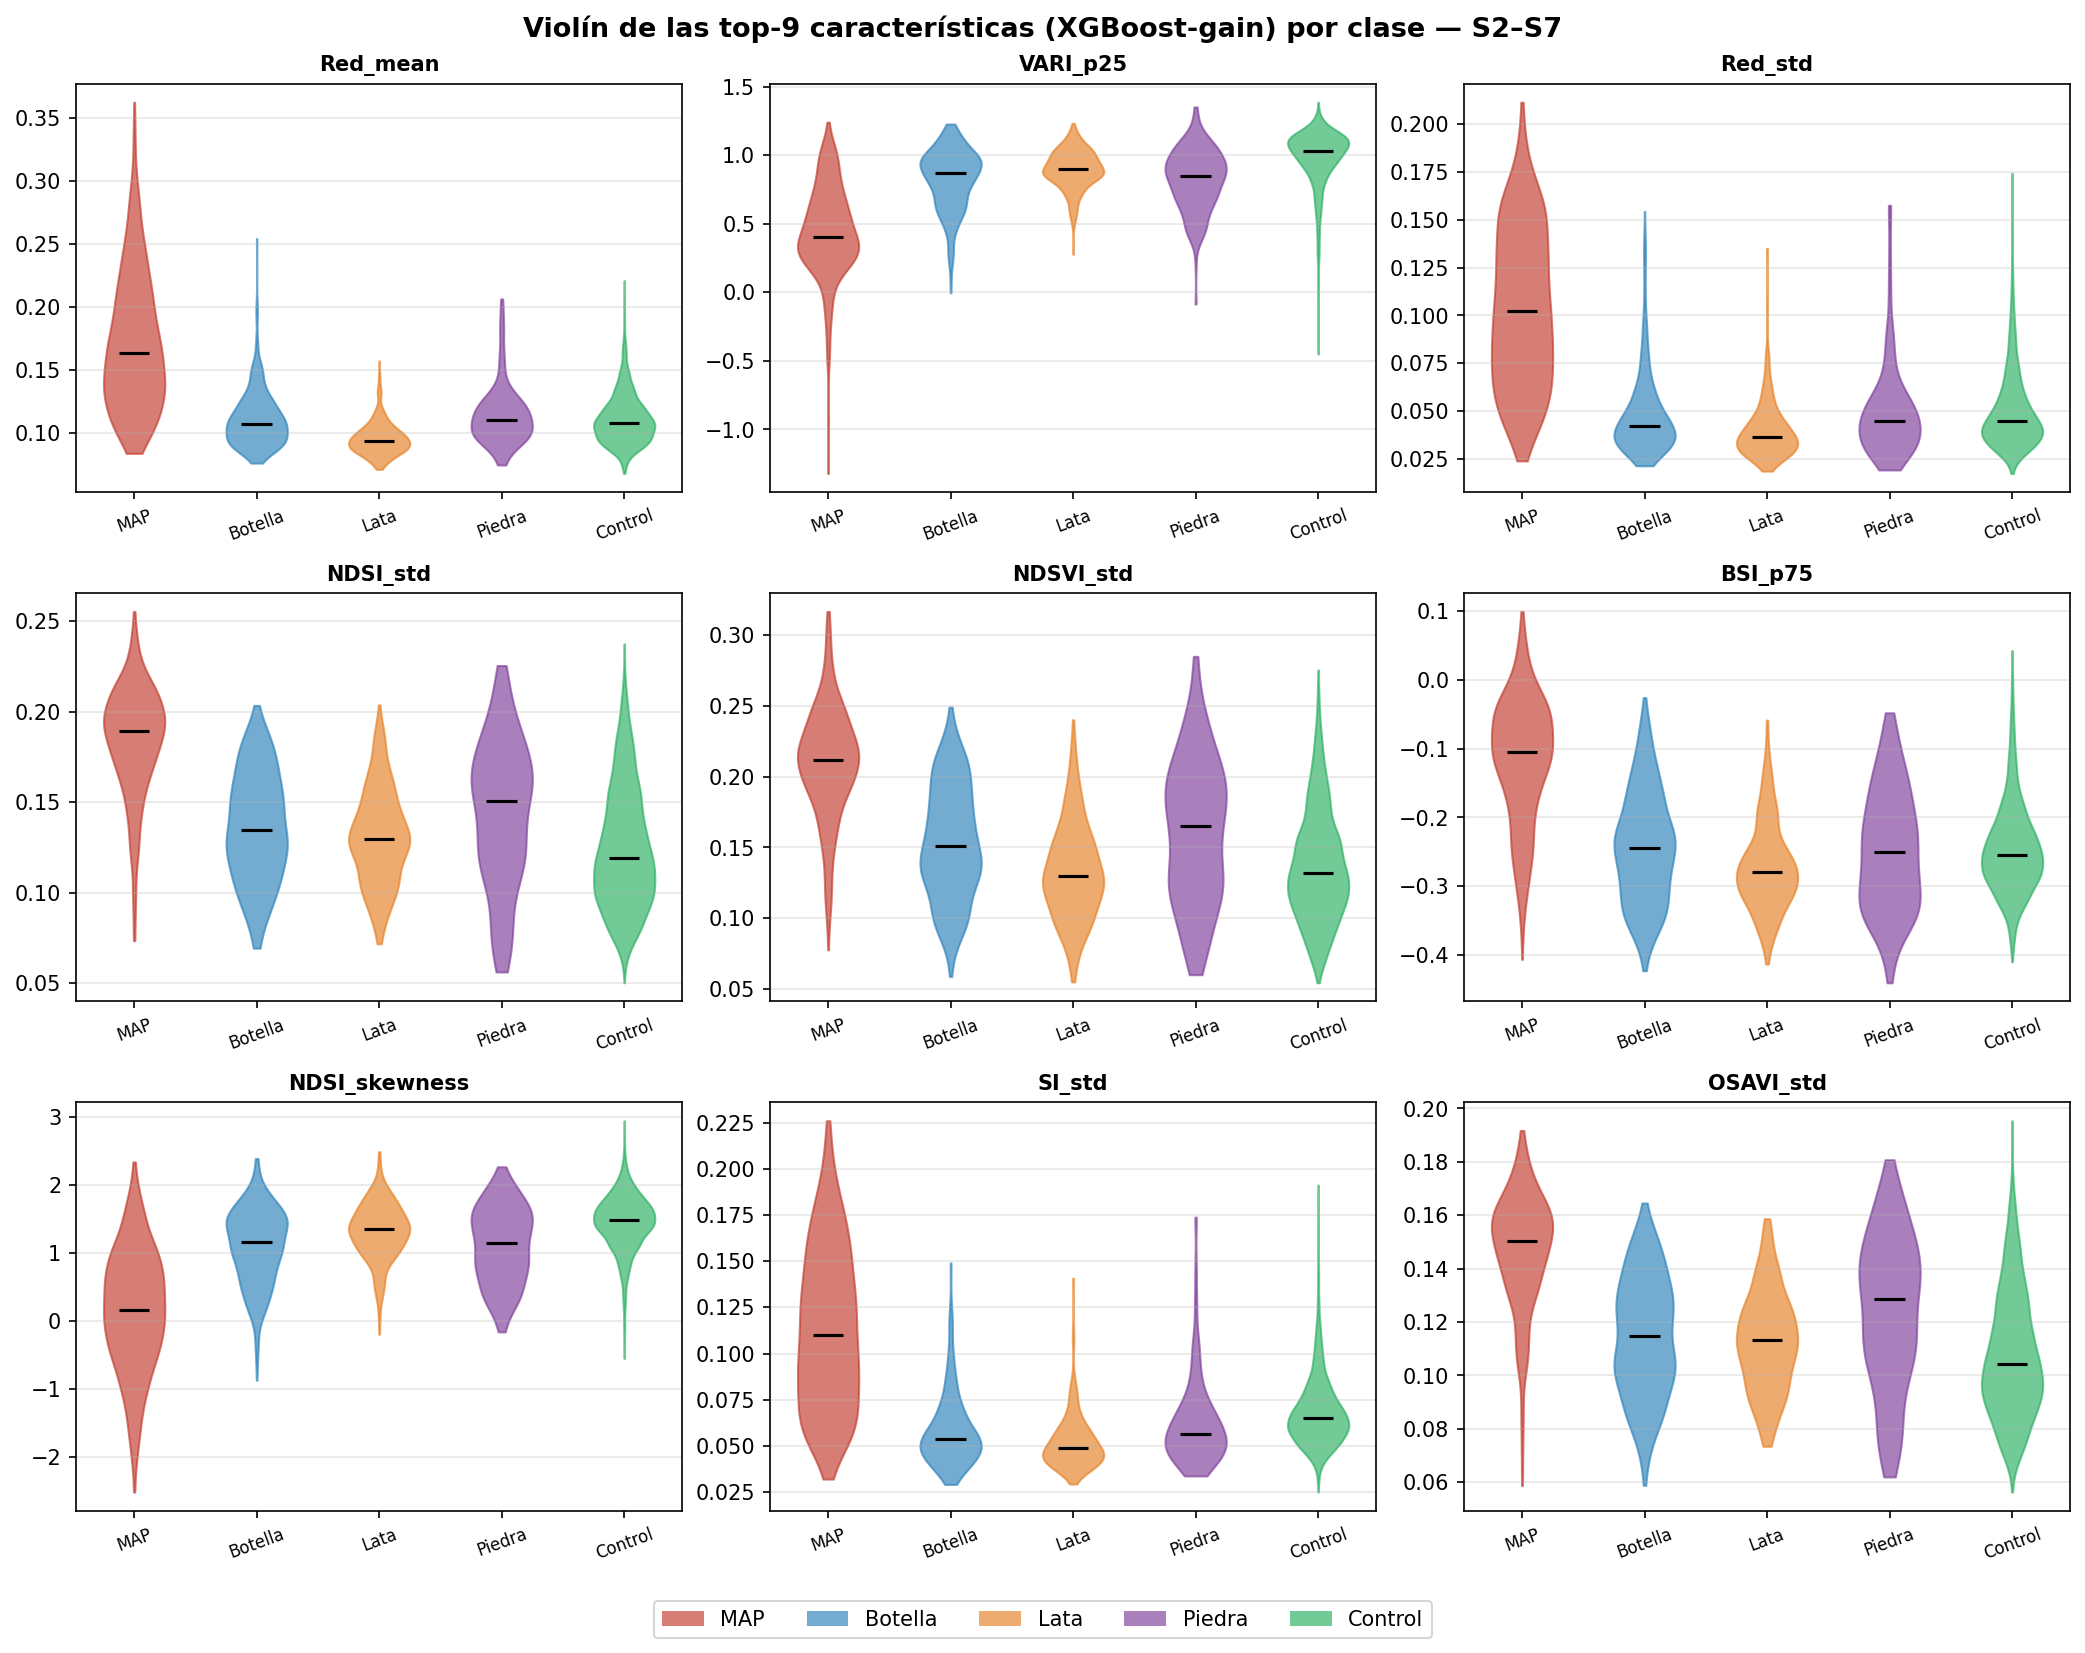
\includegraphics[width=\textwidth]{figuras/violin_top_features.png}
  \caption{Violín de las características más importantes por clase. La \ac{MAP}
    (rojo) presenta mayor desviación estándar (Red\_std, NDSI\_std, NDSVI\_std,
    SI\_std\ldots), señal de la heterogeneidad local que genera la perturbación.}
  \label{fig:violin_top}

  {\footnotesize Fuente: elaboración propia.}
\end{figure}

% -------------------------------------------------------------
\section{Comparación de clasificadores}
\label{sec:clasificadores}
\label{sec:comparacion_clasificadores}

\textbf{Objetivo.} Elegir el clasificador, evaluando rendimiento y costo
computacional.

\textbf{Metodología.} Se compararon \ac{RF}, \ac{SVM} (kernel RBF), XGBoost y
\textbf{EasyEnsemble~x10} (diez XGBoost, cada uno con un submuestreo 1:1 distinto,
probabilidades promediadas), con las 378 características y \ac{LOSO}. Los
hiperparámetros se fijaron para todos los clasificadores, garantizando una
comparación homogénea: \ac{RF} con 100 árboles y profundidad máxima~10; \ac{SVM}
con $C=1$, $\gamma=$\,\texttt{scale} y \texttt{StandardScaler} ajustado por
pliegue; XGBoost ---y cada clasificador base de EasyEnsemble--- con 200 árboles,
profundidad máxima~4, tasa de aprendizaje~0.1 y submuestreo de filas y columnas
de~0.8. Para cada clasificador se midió, además de las métricas de detección, el
tiempo de entrenamiento e inferencia como medida del costo computacional.

\begin{table}[H]
\centering
\caption{Comparación de clasificadores (378 características, \ac{LOSO}, 1:1).}
\label{tab:clasificadores}
\small
\begin{tabular}{lccccc}
\toprule
\textbf{Clasificador} & \textbf{AUC} & \textbf{Sens(0.5)} & \textbf{Spec(0.5)} &
\textbf{FP/mina} & \textbf{Inferencia} \\
\midrule
Random Forest & 0.915 $\pm$ 0.023 & 0.805 & 0.856 & 5.29 & 22.9 µs/vent. \\
SVM (RBF) & 0.929 $\pm$ 0.010 & 0.758 & 0.880 & 4.70 & 108 µs/vent. \\
XGBoost & 0.941 $\pm$ 0.014 & 0.817 & 0.885 & 4.15 & \textbf{2.6 µs/vent.} \\
\textbf{EasyEnsemble x10} & \textbf{0.945 $\pm$ 0.013} & \textbf{0.832} &
0.883 & 4.16 & 29.7 µs/vent. \\
\bottomrule
\end{tabular}

  {\footnotesize Fuente: elaboración propia.}
\end{table}

\textbf{Resultados.} Como resume la Tabla~\ref{tab:clasificadores}, \textbf{EasyEnsemble} es el mejor en \ac{AUC} (0.945) y
sensibilidad (0.832), y el más estable. La Figura~\ref{fig:matrices} presenta una matriz de
confusión por clasificador: las filas son la clase real y las columnas la
predicción del modelo, de modo que el porcentaje de cada fila indica qué fracción
de esa clase se clasificó bien (no-minas correctas en la fila superior, minas
detectadas en la inferior). EasyEnsemble domina las dos filas a la vez: detecta
más minas \emph{y} produce menos falsas alarmas (1\,684 FP, el menor).

\begin{figure}[H]
  \centering
  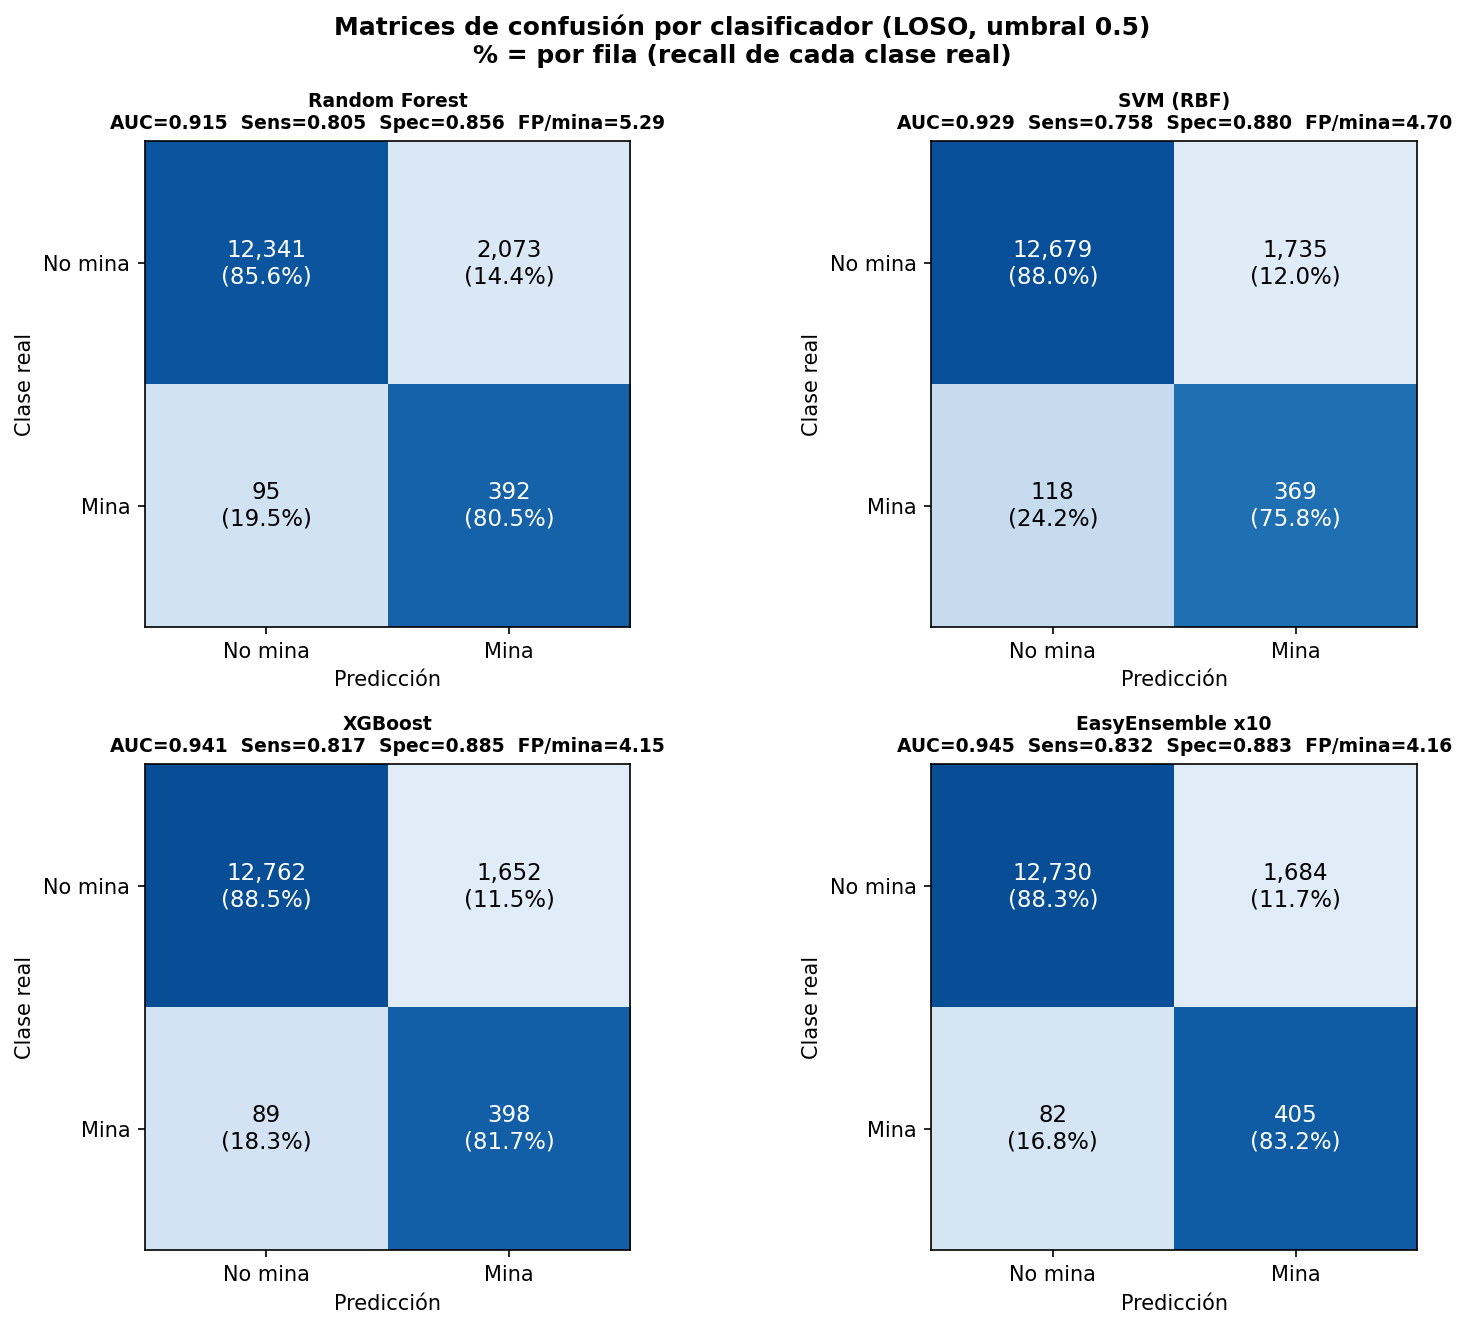
\includegraphics[width=\textwidth]{figuras/p3c_matrices.png}
  \caption{Matrices de confusión por clasificador (\ac{LOSO}, umbral~0.5;
    \% por fila = recall de cada clase). EasyEnsemble equilibra mejor ambas filas.}
  \label{fig:matrices}

  {\footnotesize Fuente: elaboración propia.}
\end{figure}

\textbf{Análisis de complejidad.} EasyEnsemble cuesta $\sim$10$\times$ más en
entrenamiento e inferencia que un solo XGBoost (son diez modelos), por una
ganancia pequeña ($+0.004$ \ac{AUC}). Sin embargo, en términos absolutos la
inferencia es trivial: $\sim$6~ms por imagen frente a $\sim$25~s de extracción.
El sobrecosto es despreciable para análisis post-captura, así que se elige
\textbf{EasyEnsemble} por sus mejores métricas; XGBoost queda como alternativa
ligera (11$\times$ más rápido, $-0.004$ \ac{AUC}) para hardware limitado.

% -------------------------------------------------------------
\section{Selección de características}
\label{sec:seleccion_k}

\textbf{Objetivo.} Definir cómo se seleccionan las características del modelo
final: con qué medida de importancia se ordenan y cuántas conservar sin perder
rendimiento.

\textbf{Metodología.} Las características se ordenan por la \textbf{importancia de
ganancia de XGBoost}, calculada dentro de cada pliegue \ac{LOSO} (consistente con
el clasificador final, sin fuga de información); para justificar esa elección se
compara contra ordenarlas por la importancia Gini de \ac{RF}. Luego se barre el
número de características $k$ con \textbf{paso uniforme de 10}
($k=10,20,\ldots,378$) y se elige, con un criterio explícito, el menor $k$ que
alcanza el 99.5\,\% del \ac{AUC} máximo (la meseta de rendimiento).

\textbf{Método de selección.} Ordenar por la ganancia de XGBoost iguala o supera a
ordenar por la importancia de \ac{RF} (Figura~\ref{fig:metodo_sel}): a $k=50$,
\ac{AUC}~0.942 frente a 0.935; a $k=100$, 0.947 frente a 0.940. Como el
clasificador final es XGBoost, ordenar con su \emph{propia} medida de importancia
es lo consistente y, además, no penaliza el rendimiento.

\begin{figure}[H]
  \centering
  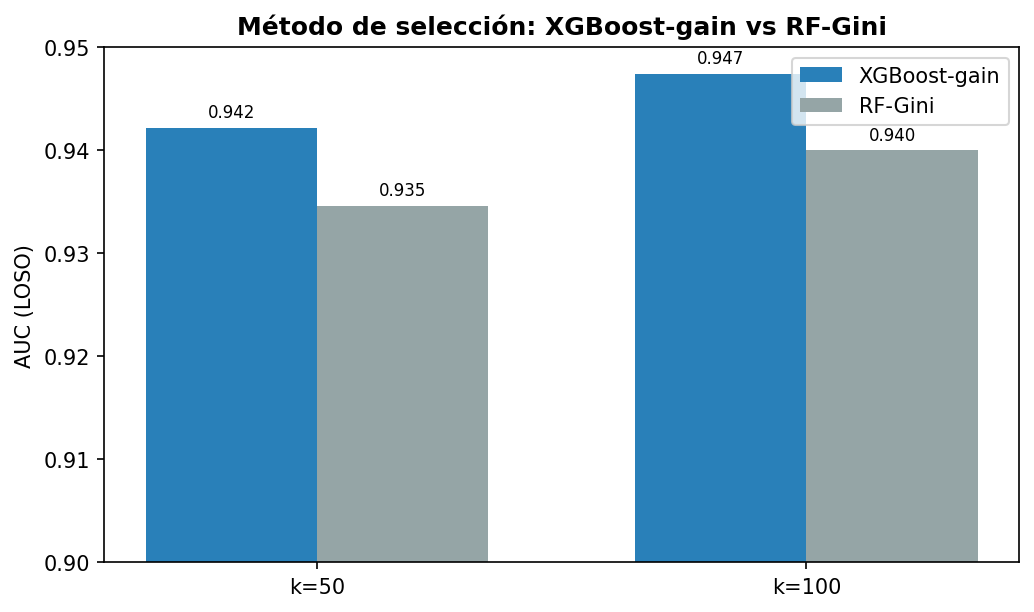
\includegraphics[width=0.62\textwidth]{figuras/p4_metodo_seleccion.png}
  \caption{Método de selección: ordenar las características por la ganancia de
    XGBoost vs.\ por la importancia Gini de \ac{RF} (\ac{AUC} \ac{LOSO}, $k=50$
    y $k=100$).}
  \label{fig:metodo_sel}

  {\footnotesize Fuente: elaboración propia.}
\end{figure}

\textbf{Número de características.} La Figura~\ref{fig:barrido_k} traza el \ac{AUC}
(y la sensibilidad y especificidad) frente a $k$: la curva sube rápido y luego se
aplana formando una meseta. Bajo el criterio anterior, el menor $k$ admisible es
$k=60$. Se elige \textbf{$k=70$} por ser el punto de la meseta que \emph{domina} a
$k=60$ en todas las métricas (AUC 0.947, Sens 0.823, Spec 0.884, FP/mina 4.16
vs.\ 0.944/0.819/0.882/4.26), priorizando la sensibilidad ---la métrica crítica en
detección de minas--- por solo diez características más. El criterio alternativo de
\emph{importancia acumulada} se descarta: como la importancia está repartida entre
muchas características, exigir el 90\,\% acumulado llevaría a $k=235$ ---casi
todas--- para el mismo \ac{AUC}.

\begin{figure}[H]
  \centering
  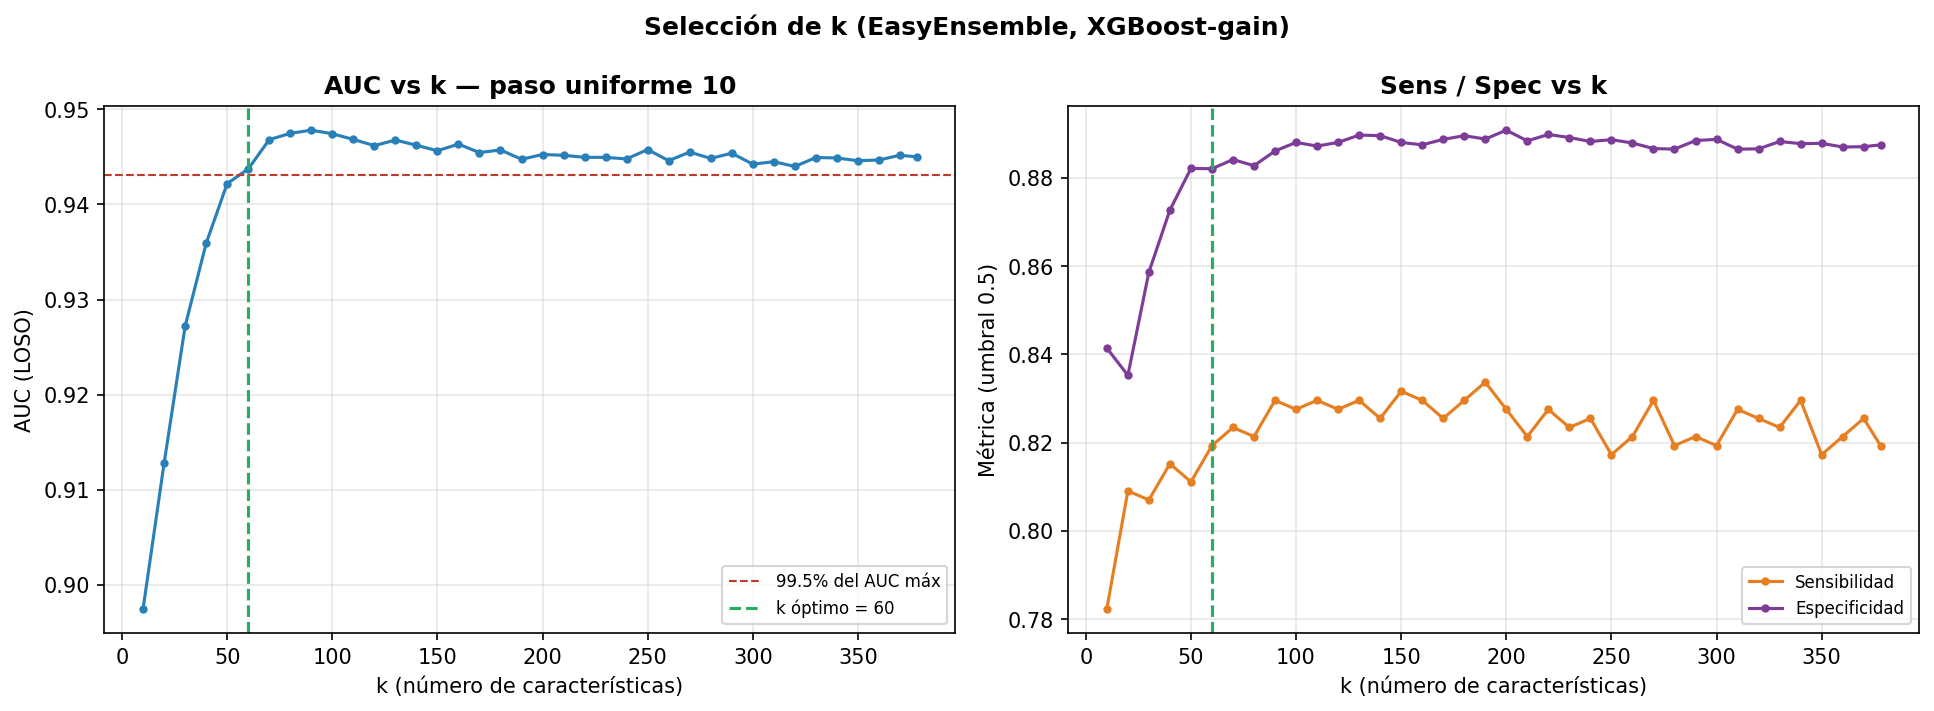
\includegraphics[width=\textwidth]{figuras/p4_barrido_k.png}
  \caption{Selección de $k$ (EasyEnsemble, XGBoost-gain). \textit{Izquierda:}
    \ac{AUC} vs.\ $k$ con el criterio del 99.5\,\%. \textit{Derecha:}
    sensibilidad y especificidad vs.\ $k$.}
  \label{fig:barrido_k}

  {\footnotesize Fuente: elaboración propia.}
\end{figure}

% -------------------------------------------------------------
\section{Modelo final: métricas con LOSO por fold}
\label{sec:modelo_final}

\textbf{Objetivo.} Reportar el rendimiento del modelo final ---EasyEnsemble~x10,
top-70 características--- bajo \ac{LOSO}.

\textbf{Metodología.} Se aplica el modelo final ---EasyEnsemble~x10 con las
top-70 características seleccionadas por ganancia de XGBoost dentro de cada
pliegue--- bajo \ac{LOSO}, y se reportan las métricas por sesión a umbral~0.5.

\begin{table}[H]
\centering
\caption{Métricas \ac{LOSO} por fold del modelo final (EasyEnsemble~x10,
         top-70, umbral~0.5).}
\label{tab:modelo_final}
\small
\begin{tabular}{lccccccc}
\toprule
\textbf{Fold} & \textbf{AUC} & \textbf{Sens} & \textbf{Spec} &
\textbf{TP} & \textbf{FN} & \textbf{FP} & \textbf{TN} \\
\midrule
S2 & 0.936 & 0.827 & 0.898 & 62 & 13 & 191 & 1\,678 \\
S3 & 0.946 & 0.964 & 0.669 & 81 & 3  & 831 & 1\,677 \\
S4 & 0.942 & 0.770 & 0.921 & 67 & 20 & 198 & 2\,307 \\
S5 & 0.950 & 0.815 & 0.916 & 66 & 15 & 212 & 2\,298 \\
S6 & 0.958 & 0.872 & 0.938 & 68 & 10 & 156 & 2\,356 \\
S7 & 0.948 & 0.695 & 0.967 & 57 & 25 & 82  & 2\,428 \\
\midrule
\textbf{Prom.} & \textbf{0.947} & \textbf{0.823} & \textbf{0.884} &
401 & 86 & 1\,670 & 12\,744 \\
\bottomrule
\end{tabular}

  {\footnotesize Fuente: elaboración propia.}
\end{table}

\textbf{Resultados.} El modelo final alcanza \textbf{AUC~=~0.947, sensibilidad
82.3\,\%, especificidad 88.4\,\% y $\sim$4.2 falsos positivos por mina}. En la
matriz de confusión (Figura~\ref{fig:confusion_final}), de las 487 minas reales
el sistema detecta 401 y se le escapan 86; de las 14\,414 ventanas sin mina,
12\,744 se rechazan correctamente y 1\,670 producen falsas alarmas. El porcentaje
de cada fila es el recall de esa clase (sensibilidad en la fila de mina,
especificidad en la de no-mina).

\begin{figure}[H]
  \centering
  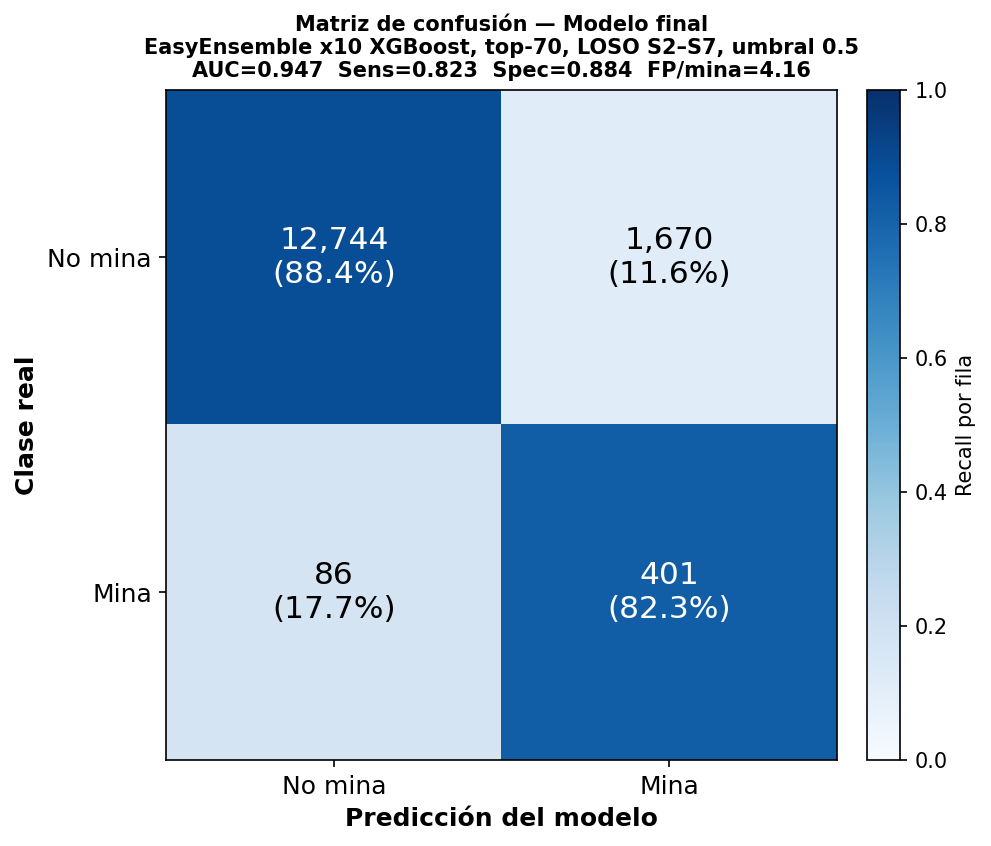
\includegraphics[width=0.62\textwidth]{figuras/p5_matriz_confusion.png}
  \caption{Matriz de confusión del modelo final (EasyEnsemble~x10, top-70,
    \ac{LOSO} S2--S7, umbral~0.5). Conteos reales; el porcentaje de cada fila es
    el recall de esa clase.}
  \label{fig:confusion_final}

  {\footnotesize Fuente: elaboración propia.}
\end{figure}

\textbf{Análisis.} El comportamiento varía entre sesiones (Tabla~\ref{tab:modelo_final}): S3
detecta casi todas las minas (Sens 0.964) pero genera muchas falsas alarmas
(Spec 0.669), mientras que S7 es lo contrario (Spec 0.967, Sens 0.695). Esta
variabilidad refleja que es un \emph{problema difícil}: las clases se solapan, no
hay un discriminador marcado y las condiciones de cada sesión afectan el balance
entre detección y falsas alarmas. Aun así, el \ac{AUC} se mantiene alto y estable
($0.947 \pm 0.007$) en las seis sesiones.

Para ilustrar el comportamiento del modelo sobre imágenes que \emph{no vio durante
el entrenamiento}, la Figura~\ref{fig:mapa} aplica el modelo final a dos imágenes de
la Sesión~2, predichas ---bajo \ac{LOSO}--- por el modelo entrenado únicamente con
las otras cinco sesiones. En la \textbf{zona de mina} (fila superior) la alta
probabilidad se concentra sobre la \ac{MAP} ---sus nueve ventanas se detectan--- y
los falsos positivos quedan en el borde difuso del suelo perturbado que la rodea
(su análisis se presenta en la Figura~\ref{fig:fp_espacial}, Sección~\ref{sec:fp_objetos}). En la \textbf{zona de
control} (fila inferior, sin mina enterrada) el modelo permanece prácticamente
apagado: solo 2 de 216 ventanas superan el umbral. El sistema enciende donde hay
mina y se mantiene silencioso donde no la hay, sobre imágenes nunca vistas en
entrenamiento.

\begin{figure}[H]
  \centering
  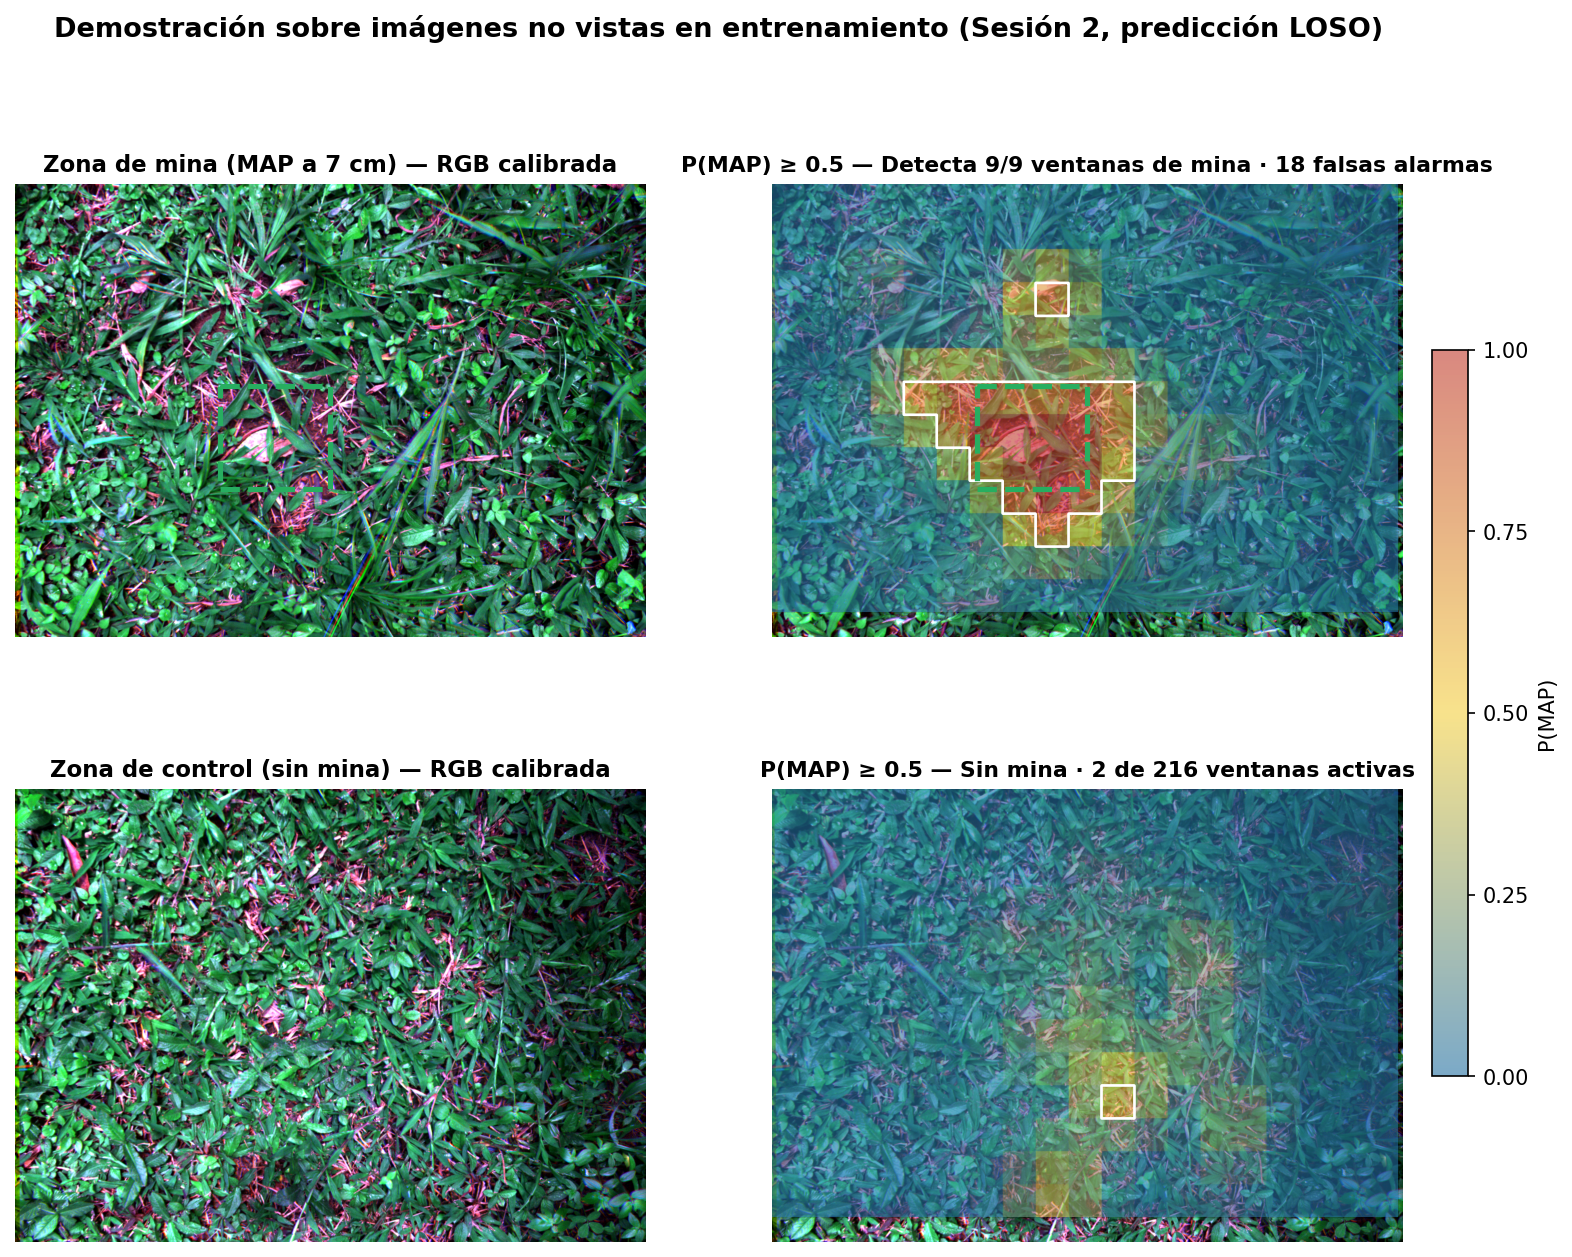
\includegraphics[width=\textwidth]{figuras/demo_no_vista.png}
  \caption{Demostración del modelo final sobre dos imágenes no vistas en
    entrenamiento (Sesión~2; predicción \ac{LOSO}, es decir, el modelo se entrenó
    sin la Sesión~2). \textit{Fila superior:} zona de mina (\ac{MAP} a 7~cm).
    \textit{Fila inferior:} zona de control sin mina. \textit{Izquierda:} RGB
    calibrada (bounding box de la \ac{MAP} en verde discontinuo).
    \textit{Derecha:} probabilidad de \ac{MAP} superpuesta (azul = baja, rojo =
    alta) con el contorno del umbral~0.5. La probabilidad alta se concentra sobre
    la mina y queda casi ausente en la zona de control.}
  \label{fig:mapa}

  {\footnotesize Fuente: elaboración propia.}
\end{figure}

% -------------------------------------------------------------
\section{Generalización a emplazamientos no vistos}
\label{sec:lozo}

\textbf{Objetivo.} La validación \ac{LOSO} deja fuera una sesión, pero las mismas
ocho zonas físicas de mina se fotografían en las seis sesiones. Cabe preguntarse si
el modelo aprende la \emph{firma de la mina} o memoriza esos ocho emplazamientos.
Para distinguirlo se evalúa una validación \emph{leave-one-zone-out} (LOZO): se deja
fuera del entrenamiento una zona de mina completa (sus seis sesiones) y se prueba
sobre ella, de modo que el modelo nunca vio ese emplazamiento.

\textbf{Metodología.} Mismo modelo final que en la
Sección~\ref{sec:modelo_final} (EasyEnsemble~x10 con las top-70 características
seleccionadas por ganancia de XGBoost dentro de cada pliegue, submuestreo 1:1); solo
cambia el agrupamiento del pliegue ---por emplazamiento físico en lugar de por
sesión--- para una comparación controlada.

\begin{table}[H]
\centering
\caption{Comparación de esquemas de validación (modelo final: EasyEnsemble~x10, top-70 características).}
\label{tab:lozo}
\small
\begin{tabular}{lc}
\toprule
\textbf{Esquema de validación} & \textbf{AUC} \\
\midrule
\ac{LOSO} (deja una sesión fuera) & $0.947 \pm 0.007$ \\
LOZO (deja un emplazamiento fuera) & $0.933 \pm 0.021$ \\
\bottomrule
\end{tabular}

  {\footnotesize Fuente: elaboración propia.}
\end{table}

\textbf{Resultados.} Al dejar fuera un emplazamiento completo, el \ac{AUC} apenas
desciende ($0.947 \to 0.933$, $-0.014$), dentro de la variabilidad entre pliegues,
y se mantiene entre 0.899 y 0.961 en las ocho zonas. La caída es marginal: si el
modelo memorizara los ocho sitios, su rendimiento sobre un emplazamiento no visto se
desplomaría, lo que no ocurre. Esto indica que el modelo aprende la firma espectral
del fenómeno ---perturbación del suelo y estrés vegetal--- y \textbf{generaliza a emplazamientos no vistos} bajo las condiciones ya
observadas, de forma complementaria a la robustez ante nuevas condiciones de
captura que evalúa la validación \ac{LOSO}. La comparación se centra en el \ac{AUC} por ser independiente tanto del umbral como de la composición del conjunto de prueba.

% -------------------------------------------------------------
\section{Rendimiento por sesión y condiciones de captura}
\label{sec:condiciones}

\textbf{Objetivo.} Evaluar si la hora, la humedad o la radiación solar afectan el
\ac{AUC}.

\textbf{Metodología.} Se relaciona el \ac{AUC} por sesión del modelo final con las
condiciones de captura registradas. Con solo seis sesiones se hace una inspección
cualitativa, sin coeficiente de correlación (que carecería de potencia estadística).

\begin{table}[H]
\centering
\caption{\ac{AUC} por sesión vs.\ condiciones de captura (ordenado por hora).}
\label{tab:condiciones}
\small
\begin{tabular}{ccccc}
\toprule
\textbf{Sesión} & \textbf{Hora} & \textbf{HR (\%)} &
\textbf{Rad. (W/m\textsuperscript{2})} & \textbf{AUC} \\
\midrule
S6 & 07:30 & 84.5 & 161.5 & 0.958 \\
S3 & 12:34 & 60.7 & 346.7 & 0.946 \\
S2 & 13:10 & 72.8 & 778.7 & 0.936 \\
S7 & 16:40 & 65.5 & 143.9 & 0.948 \\
S5 & 17:17 & 63.6 & 73.3  & 0.950 \\
S4 & 17:21 & 61.8 & 64.5  & 0.942 \\
\bottomrule
\end{tabular}

  {\footnotesize Fuente: elaboración propia.}
\end{table}

\textbf{Análisis.} Según la Tabla~\ref{tab:condiciones}, el \ac{AUC} varía poco (0.936--0.958) y \emph{no} sigue un
patrón con la hora ni la radiación: S6 a las 07:30 (sol rasante) obtiene el
\ac{AUC} más alto, comparable al de mediodía. La inspección cualitativa indica
que la firma multiespectral es \emph{estable} dentro del rango
horario del protocolo, a diferencia de la señal térmica que requiere ventanas
temporales específicas.

% -------------------------------------------------------------
\section{Rendimiento por profundidad de enterramiento}
\label{sec:profundidad}

\textbf{Objetivo.} Analizar el desempeño según la profundidad (1, 3, 5, 7~cm).

\textbf{Metodología.} Las ventanas de prueba del modelo final se reagrupan por la
profundidad de su zona y se recalculan las métricas en cada subgrupo; es el mismo
modelo, sin reentrenar.

\begin{table}[H]
\centering
\caption{Métricas \ac{LOSO} por profundidad (modelo final).}
\label{tab:profundidad}
\small
\begin{tabular}{cccc}
\toprule
\textbf{Profundidad} & \textbf{AUC} & \textbf{Sens} & \textbf{Spec} \\
\midrule
\SI{1}{cm} & 0.942 & 0.875 & 0.858 \\
\SI{3}{cm} & 0.914 & 0.880 & 0.813 \\
\SI{5}{cm} & 0.928 & 0.835 & 0.855 \\
\SI{7}{cm} & 0.915 & 0.707 & 0.923 \\
\bottomrule
\end{tabular}

  {\footnotesize Fuente: elaboración propia.}
\end{table}

\textbf{Análisis.} La \textbf{sensibilidad cae con la profundidad} (Tabla~\ref{tab:profundidad})
($0.875$ a \SI{1}{cm} $\to$ $0.707$ a \SI{7}{cm}), coherente con la física: a
menor profundidad, mayor perturbación del suelo y del estrés vegetal, señales más
detectables. En la Figura~\ref{fig:profundidad}, la línea negra es el promedio
\ac{LOSO} del \ac{AUC} y las de colores cada sesión: el \ac{AUC} se mantiene estable
(entre 0.91 y 0.94), pues la pérdida de rendimiento con la profundidad se manifiesta
en la sensibilidad (Tabla~\ref{tab:profundidad}), no en el \ac{AUC}. A \SI{7}{cm} la detección es la más
difícil, aunque el \ac{AUC} permanece muy por encima del azar. Esto refuerza que
la señal proviene de la perturbación superficial del enterramiento.

\begin{figure}[H]
  \centering
  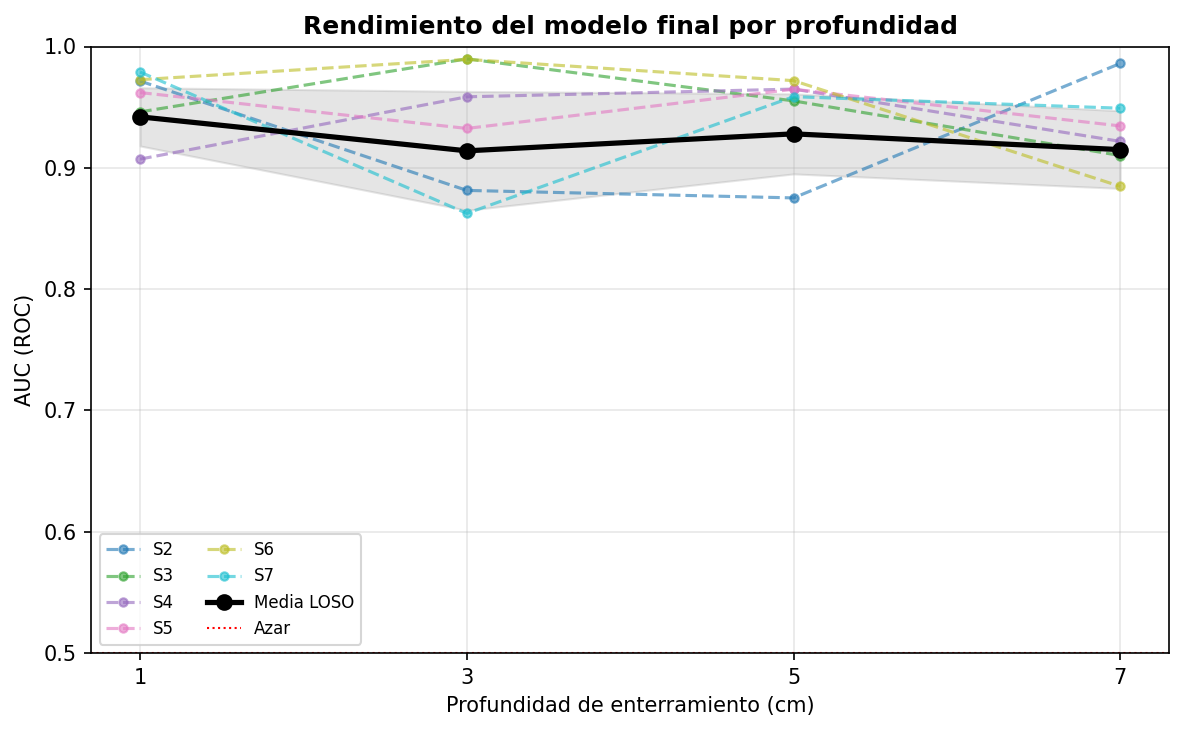
\includegraphics[width=0.85\textwidth]{figuras/p7_profundidad.png}
  \caption{\ac{AUC} por profundidad. Línea negra: promedio \ac{LOSO};
    líneas de color: cada sesión.}
  \label{fig:profundidad}

  {\footnotesize Fuente: elaboración propia.}
\end{figure}

% -------------------------------------------------------------
\section{Falsos positivos vs objetos de interferencia}
\label{sec:fp_objetos}
\label{sec:analisis_fp}

\textbf{Objetivo.} Determinar si los objetos de interferencia (botella, lata,
piedra) son la causa de los falsos positivos.

\textbf{Metodología.} Cada falso positivo del modelo final (ventana sin mina
clasificada como mina) se etiqueta según dónde cae ---sobre un objeto de
interferencia o sobre el fondo de suelo perturbado---, y se compara contra una
variante que fuerza una cuota de objetos en el submuestreo.

\textbf{Resultados.} De los 1\,363 falsos positivos en zonas de mina, solo el
\textbf{6.8\,\% caen sobre objetos} (Botella 57, Lata 17, Piedra 19) y el
\textbf{93.2\,\% sobre el fondo} ---el suelo perturbado alrededor de la mina,
cuyo borde difuso se extiende más allá del bounding box
(Figura~\ref{fig:fp_comp}). El objeto que más confunde es la \textbf{botella}.

\begin{figure}[H]
  \centering
  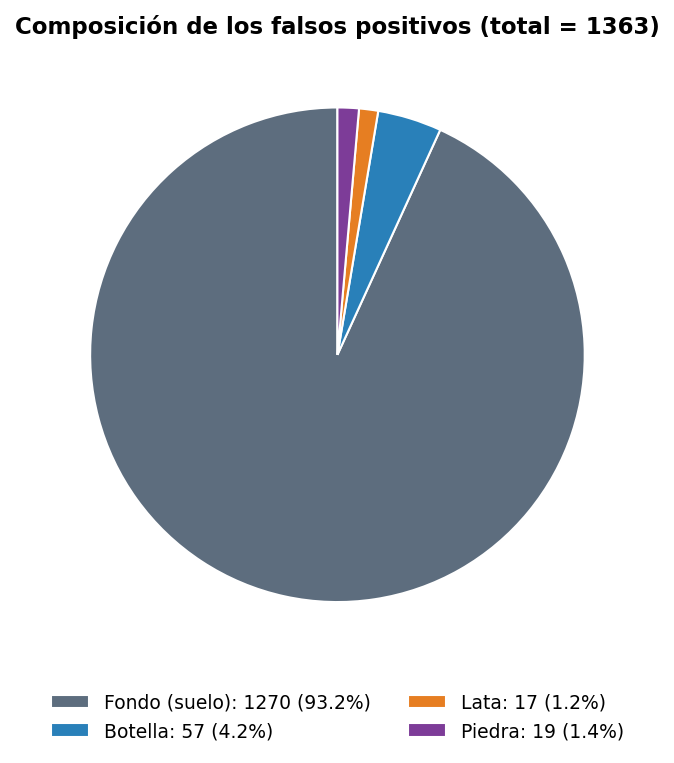
\includegraphics[width=0.62\textwidth]{figuras/p8_composicion.png}
  \caption{Composición de los falsos positivos del modelo final: el 93\,\% cae
    sobre el fondo (suelo perturbado) y solo el 6.8\,\% sobre objetos.}
  \label{fig:fp_comp}

  {\footnotesize Fuente: elaboración propia.}
\end{figure}

\textbf{Dónde falla el sistema.} Como casi todos los falsos
positivos están en suelo perturbado/desnudo y no en los objetos, el sistema
\emph{falla más en zonas de suelo removido o sin vegetación}, que se parecen a la
perturbación de una mina. En cambio, en \emph{áreas de vegetación homogénea} su
desempeño es mejor. Es una limitación honesta y a la vez una guía de uso. La
Figura~\ref{fig:fp_espacial} lo ilustra sobre una imagen: los falsos positivos se
reparten por el suelo de la zona y solo unos pocos caen cerca de los objetos.

\begin{figure}[H]
  \centering
  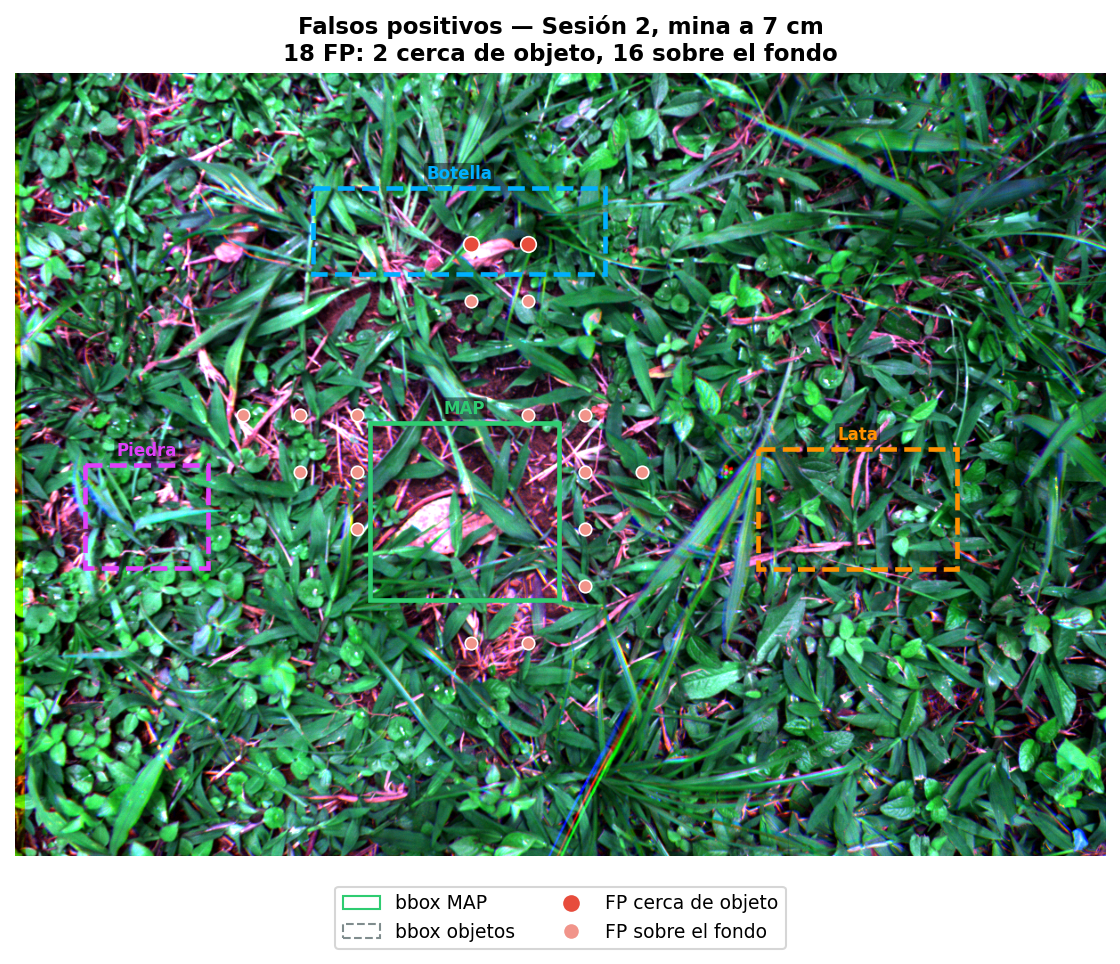
\includegraphics[width=0.78\textwidth]{figuras/fp_ejemplo.png}
  \caption{Ejemplo de falsos positivos sobre una imagen (Sesión~2, mina a 7~cm;
    predicción \ac{LOSO}, imagen no usada en el entrenamiento de ese fold). De los
    18 falsos positivos, solo 2 caen cerca de un objeto y 16 sobre el fondo,
    coherente con el conjunto.}
  \label{fig:fp_espacial}

  {\footnotesize Fuente: elaboración propia.}
\end{figure}

\textbf{Experimento: cuota de objetos.} Se evaluó forzar una cuota de objetos
(\emph{hard-negative mining}) en el submuestreo, para que el clasificador
aprendiera mejor a rechazarlos. La comparación limpia mostró que \textbf{no
ayuda} (Figura~\ref{fig:fp_cuota}): no reduce los FP sobre objetos (93 vs.\ 97)
y empeora levemente las métricas globales. La razón es coherente con lo anterior:
los objetos no son la fuente principal de falsas alarmas, así que
sobre-representarlos no ataca el problema. El modelo final usa submuestreo
aleatorio 1:1 (sin cuota). Un clasificador multiclase que distinga explícitamente
la \ac{MAP} de estos objetos queda como trabajo futuro
(Sección~\ref{sec:trabajos_futuros}).

\begin{figure}[H]
  \centering
  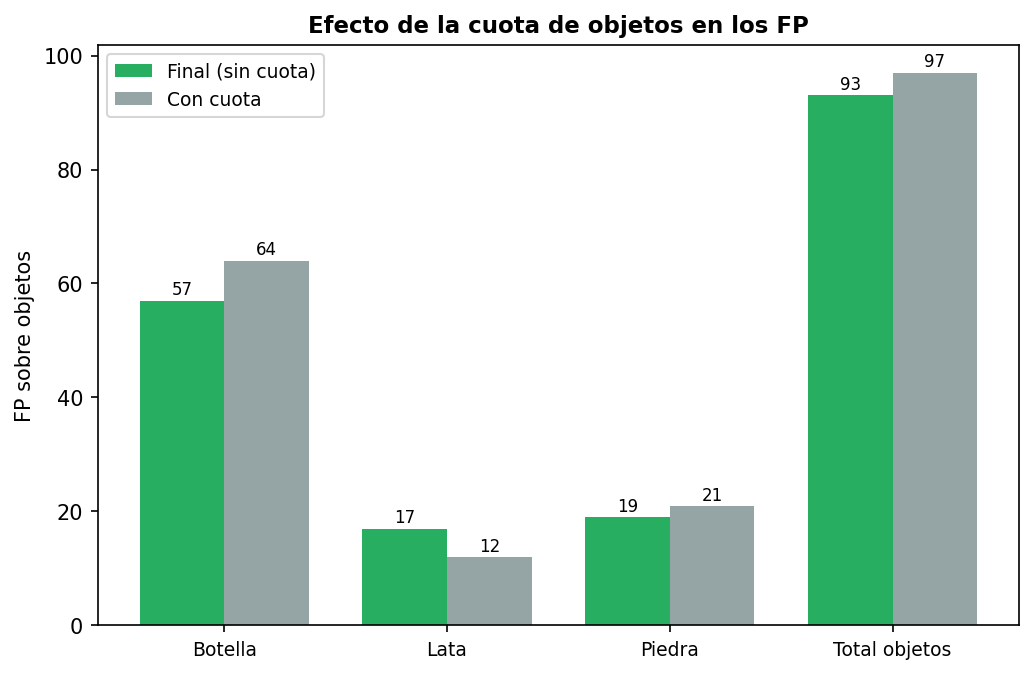
\includegraphics[width=0.75\textwidth]{figuras/p8_cuota.png}
  \caption{Efecto de la cuota de objetos: forzarla no reduce los FP sobre objetos
    (93 vs.\ 97) frente al modelo final sin cuota.}
  \label{fig:fp_cuota}

  {\footnotesize Fuente: elaboración propia.}
\end{figure}

% -------------------------------------------------------------
\section{Discusión general}
\label{sec:discusion}

La Tabla~\ref{tab:progresion} resume la progresión metodológica.

\begin{table}[H]
\centering
\caption{Progresión metodológica (S2--S7, umbral~0.5).}
\label{tab:progresion}
\small
\begin{tabular}{lccc}
\toprule
\textbf{Configuración} & \textbf{AUC} & \textbf{Sens} & \textbf{FP/mina} \\
\midrule
Random Forest, 378 características (base) & 0.915 & 0.805 & 5.29 \\
XGBoost, 378 características & 0.941 & 0.817 & 4.15 \\
EasyEnsemble, 378 características & 0.945 & 0.832 & 4.16 \\
\textbf{EasyEnsemble, top-70 (modelo final)} & \textbf{0.947} & \textbf{0.823} &
\textbf{4.16} \\
\bottomrule
\end{tabular}

  {\footnotesize Fuente: elaboración propia.}
\end{table}

El sistema final alcanza \textbf{AUC~=~0.947} con \ac{LOSO}, una ganancia de
$+0.032$ sobre la línea base (\ac{RF}, 0.915). El \emph{pipeline} completo
(calibración, alineación, extracción e inferencia) tarda entre 5 y 8~minutos por
sesión, suficiente para análisis post-captura en campo.

\textbf{Comparación con el estado del arte multiespectral.} El trabajo más
comparable es el de Silva~\etal{} \cite{silva2019}, que también detecta minas
enterradas con una cámara multiespectral y características estadísticas. Sin
embargo, sus experimentos se realizaron en \emph{cajones de arena de laboratorio}
y campo controlado, con minas enterradas pocos minutos antes de la captura
---\emph{sin señal crónica acumulada}--- y un dataset balanceado artificialmente
con partición aleatoria, alcanzando 97\,\% de exactitud. Notablemente, su sistema
\emph{no detectaba la perturbación del suelo}: justamente la señal que este
trabajo explota. En contraste, aquí se trabaja en \textbf{campo real con
vegetación en crecimiento libre ($\sim$6 meses), minas enterradas a 1--7~cm con
señal crónica, desbalance real 30:1 y validación \ac{LOSO} sin fuga de datos}.
Qiu~\etal{} \cite{qiu2023} usan una cámara multiespectral en \ac{UAV} con
\ac{NIR} y Red Edge (confirmando el valor de esas bandas), pero detectan minas en
\emph{superficie} (visibles) con una red convolucional; aquí las minas están
\emph{enterradas} (invisibles) y se detectan por su señal indirecta.

\subsection{Relación con el trabajo previo del grupo PSI}

Tenorio~\etal{} \cite{tenorio2024} es el antecedente directo dentro del grupo
\ac{PSI}: termografía infrarroja sobre \ac{UAV}, mismo terreno y tipo de mina,
con sensibilidad del 82.4\,\%. La sensibilidad obtenida aquí (82.3\,\%) es de un
nivel similar, pero \textbf{ambos trabajos no son directamente comparables}: miden
fenómenos físicos distintos ---el contraste térmico del enterramiento frente al
estrés vegetal y la anomalía del suelo---, con sensores y regímenes de validación
diferentes; además, la sensibilidad reportada corresponde en cada caso a un punto
de operación particular ---no a una medida global como el \ac{AUC}---, de modo que
dos valores cercanos no implican un rendimiento equivalente.
Los trabajos son \textbf{complementarios}: la señal térmica es aguda pero
depende de una ventana temporal estrecha (hora del día, condiciones de captura),
mientras que la señal multiespectral es más estable en el tiempo por basarse en un
efecto crónico. Una diferencia experimental clave es
que en este trabajo los \textbf{objetos de interferencia se incluyeron a
propósito} (botella, lata y piedra enterradas a la misma profundidad que la mina)
como variable controlada para medir la confusión, mientras que el estudio térmico
solo contaba con los objetos naturalmente presentes en la zona (principalmente
piedras). Por eso, fusionar ambas modalidades ---señal térmica aguda y señal
multiespectral crónica--- es una línea de trabajo natural para el grupo.
